\documentclass[12pt]{article}
\usepackage{hyperref}
\usepackage{listings}
\usepackage{biblatex}
\usepackage{tikz}
\usepackage{refstyle}
\usepackage{mathabx}
\usepackage{amssymb}
\usepackage{caption}
\usepackage{float}
\usepackage{graphicx}
\usepackage{graphics}
\usepackage{enumitem}
\usepackage{kpfonts}
\usepackage{amsmath}\usepackage{subfig}\graphicspath{{/Home/module2/geometry/math.jpeg}}

\newcommand{\abs}[1]{\lvert#1\rvert}
\newcommand{\norm}[1]{\lVert#1\rVert}
\providecommand{\sbrak}[1]{\ensuremath{{}\left[#1\right]}}
\providecommand{\brak}[1]{\ensuremath{\left(#1\right)}}
\providecommand{\cbrak}[1]{\ensuremath{\left\{#1\right\}}}
\newcommand{\myvec}[1]{\ensuremath{\begin{pmatrix}#1\end{pmatrix}}}
\newcommand{\myaugvec}[2]{\ensuremath{\begin{amatrix}{#1}#2\end{amatrix}}}
\newcommand{\mydet}[1]{\ensuremath{\begin{vmatrix}#1\end{vmatrix}}}

\begin{document}
\title{\textbf{MATH-COMPUTING}}
\maketitle
\begin{enumerate}
   
    \item \textbf{Question(MATH-12.10.5.17):}
    Let $\vec{a}$ and $\vec{b}$ be two unit vectors and $\theta$ is the angle between them. Then $\vec{a}$+$\vec{b}$ is a unit vector.
    
 \begin{enumerate}[label=(\Alph*)]                     
 \item $\theta=\frac{\pi}{4}$
 \item $\theta=\frac{\pi}{3}$
  \item $\theta=\frac{\pi}{2}$
   \item $\theta=\frac{2\pi}{3}$
   \end{enumerate}

 \textbf{solution:}

Assuming the co-ordinates:\\
{A}=\myvec{-2.31 \\ 3.98},\,
{B}=\myvec{0\\0},\,
{c}=\myvec{1.69\\0}\\

To find angle B in a triangle ABC:\\
$\cos{B} \triangleq \frac{({A}-{B})\top({C}-{B})}{\norm{{A}-{B}}\norm{{C}-{B}}}$\\

{A} - {B} = \myvec{-2.31 \\ 3.98}-\myvec{0 \\ 0} = \myvec{ -2.31\\ 3.98 }\\
{C} - {B} = \myvec{1.69 \\ 0}-\myvec{0 \\ 0} = \myvec{ 1.69\\ 0 }

$\norm{{A}-{B}} \triangleq \sqrt{\brak{{A}-{B}}^{\top}\brak{{A}-{B}}}$ = $\sqrt{\brak{{-2.31}-{3.98}}{\myvec{-2.31\\3.98}}}$ = $4.60$\\
$\norm{{C}-{B}} \triangleq \sqrt{\brak{{C}-{B}}^{\top}\brak{{C}-{B}}}$ = $\sqrt{\brak{{1.69}-{0}}{\myvec{1.69\\0}}}$ = $1.69$\\

Therefore:\\
$\cos{B}=\frac{\brak{{-2.31}-{3.98}}{\myvec{1.69\\0}}}{\brak{4.60}\brak{1.69}}$ = $\frac{-3.903}{7.774}$ = ${0.501}$\\

$ {B}=\cos^{-1}\brak{0.5}$ = $120^\degree$

 \begin{figure}[!h]
        \centering
        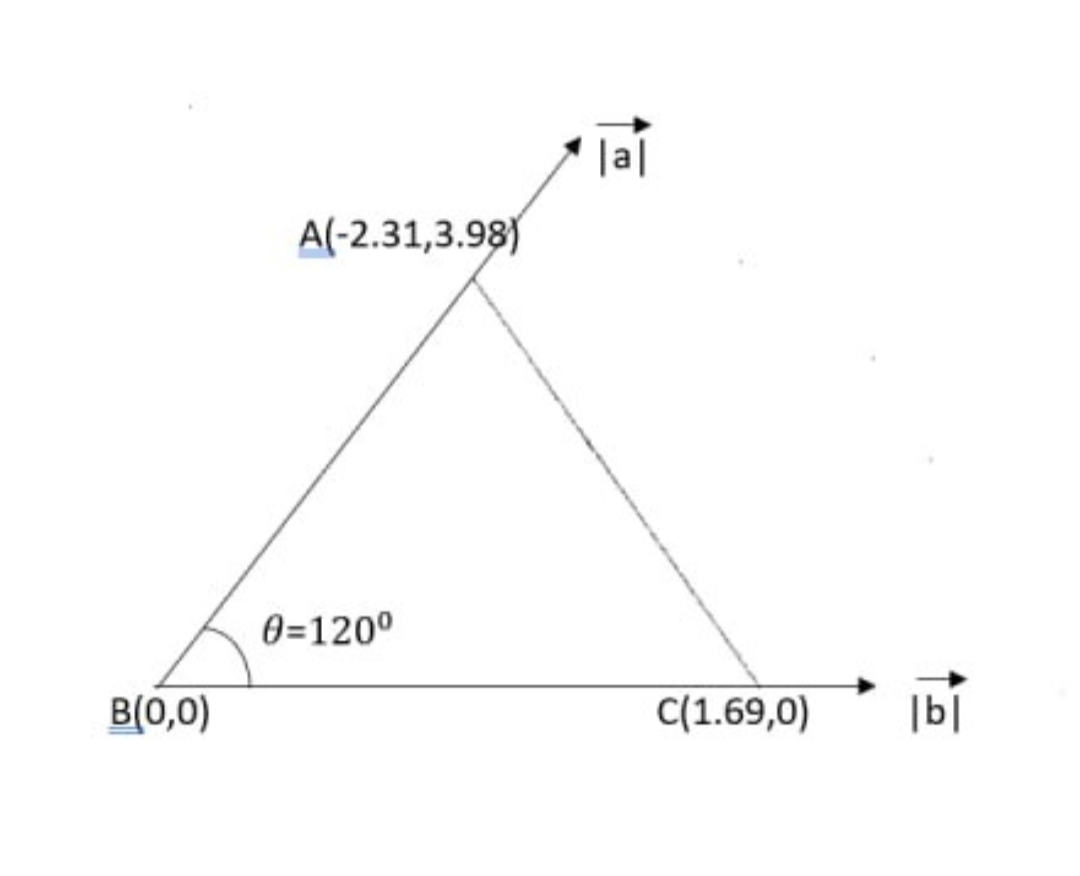
\includegraphics[width=\columnwidth]{math.jpeg}
        \caption{vectors}
        \label{fig:figure}
    \end{figure}
  \end{enumerate}
\end{document}
